\documentclass[12pt,a4paper]{article}
\usepackage[utf8]{inputenc}
\usepackage[russian]{babel}
\usepackage[OT1]{fontenc}
\usepackage{graphicx}
\usepackage{calc}
\usepackage[margin=15mm]{geometry}
\usepackage{cmap}

% условие без картинки
\newcommand{\task}[2]{
\hrule
\hbox to \textwidth {%
     \vrule
\parbox[t]{0.04\textwidth}{\smallskip \centering #1}%
     \vrule%
\hfill%
     \parbox[t]{0.93\textwidth}{\smallskip #2 \smallskip}\hfill%
\vrule
}
\hrule
    \pagebreak[2]
}

\newlength{\h}
\newsavebox{\taskbox}
\newlength{\x}
\newsavebox{\pictbox}

% условие с картинкой (картинка выравнивается по центру)
\newcommand{\taskpic}[3]{
\savebox{\taskbox}{\parbox[t]{0.93\textwidth-4.3cm}{\smallskip #2 \smallskip}}
\savebox{\pictbox}{\parbox[t]{4cm}{\smallskip \centering
     \vspace{0pt} #3 \smallskip}}
\h=\ht\taskbox
\advance\h\dp\taskbox
\x=\ht\pictbox
\advance\x\dp\pictbox
\hrule
\hbox to \textwidth {%
\vrule\parbox[t][\maxof{\h}{\x}][t]{0.04\textwidth}{ \smallskip
     \centering #1 }\vrule%
\hfill\parbox[t][\maxof{\h}{\x}][t]{0.93\textwidth-4.3cm}{\smallskip #2
     \smallskip}\hfill\vrule%
\hfill\parbox[t][\maxof{\h}{\x}][c]{4cm}{\hfil #3 \hfil}\hfill\vrule
}
\hrule
\pagebreak[2]
}
\pagestyle{empty}
\graphicspath{ {images/} }

\begin{document}

\begin{center}
\begin{Large}
\textsc{ГЦФО. 9 класс. 2014/15.}
\end{Large}
\end{center}

\small

\taskpic{34}{На концах длинной нити подвешены грузы массы $m$ каждый. Нить перекинута через два легких маленьких блока, расположенных на расстоянии $2l$ друг от друга. К ней посередине между блоками прикрепляют груз массы $2m$, и система приходит в движение. Найдите скорость грузов по истечении достаточно большого промежутка времени.}{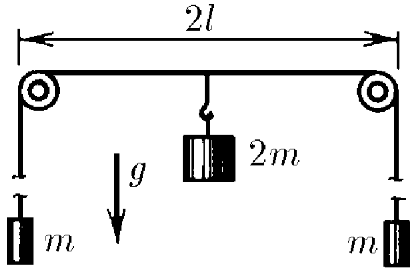
\includegraphics[width=4cm]{34}}
\taskpic{38}{Два сообщающихся сосуда, площади дна которых $S$ и $2S$, соединены трубкой L с большим резервуаром воды R. На воду в каждый сосуд положили по невесомому поршню, плотно прилегающему к стенкам. Первый поршень отвели на $x$ вверх, второй --- на $x$ вниз, и закрепили. Затем к поршням подсоединили систему нитей и блоков (см. рис.). На поршни положили грузы массами $m$ и $2m$, за нить потянули с силой $T = mg/2$. Поршни отпустили, и оказалось, что в начальный момент оба они поехали вниз. В какую сторону поехали бы поршни, если бы нить тянули с силой $mg$? Нити нерастяжимы, блоки невесомы, трением пренебречь. При движении воды по трубке уровень воды в резервуаре R практически не изменяется.}{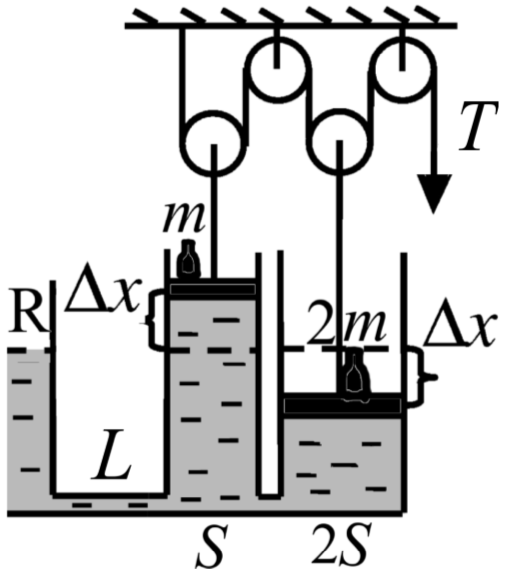
\includegraphics[width=4cm]{38}}
\taskpic{39}{Легкий жгут жесткости $k$ прикреплен к потолку, а на его конце висят два жука (см. рис.). В таком положении жгут равномерно растянут и его длина от потолка до жуков равна $l$. Потом один жук начинает карабкаться по жгуту вверх с постоянной сокростью $V$ относительно жгута. Как и с какой скоростью относительно потолка будет двигаться второй жук, который продолжает держаться за конец жгута. Считать, что каждый жук хватается за жгут в одной точке. Масса обоих жуков равна $m$, их размерами пренебречь. Ускорение свободного падения равно $g$.}{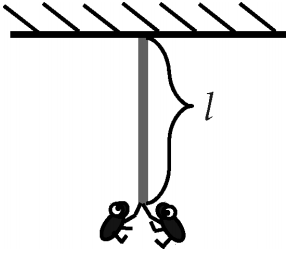
\includegraphics[width=4cm]{39}}
\taskpic{40}{Два одинаковых проводящих проволочных кольца радиуса $a$ сварили в противоположных точках O и O' как указано на рисунке. Сопротивление единицы длины проволоки равно $\lambda$. Дуги AO и BO равны, их длина $l$. Найти зависимость сопротивления между точками A и B от величины $l$.}{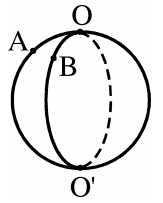
\includegraphics[width=2cm]{40}}
\task{41}{Поршень массы $M$ = 2 кг может с трением скользить внутри вертикальной неподвижной трубы. Сначала поршень прикрепили внутри трубы к потолку пружиной жесткостью $k_1$ = 20 Н/м, длина которой в нерастянутом состоянии $l_1$=60 см. Поршень расположили на уровне середины трубы, отпустили, и он остался неподвижен. Затем опыт повторили, поменяв пружину - жесткость новой пружины стала $k_2$ = 10 Н/м, а длина в нерастянутом состоянии $l_2$ = 20 см. Удивительно, но поршень в середине трубы снова остался неподвижен. При каких знчениях силы трения поршня о трубу это возможно? Влиянием воздуха пренебречь, $g$ = 10 м/с$^2$}
\taskpic{42}{Из куска покрытого изоляцией провода сопротивлением $R$ спаяли кольцо; кольцо свернули в симметричную восьмерку (с одинаковыми петельками). В середине, где провода восьмерки скрещиваются, котакта нет. Точно таким же образом изготовили вторую восьмерку. Источник тока подключают к точкам скрещивания обеих восьмерок (на рис.1 крупно показано подключение одной восьмерки): один из скрещивающихся проводов подключен к "плюсу", а другой - к "минусу". Затем полученные восьмерки спаяли друг с другом в симметричных точках $A$ и $B$(см. рис.2), сопротивление участка провода между $A$ и $B$ равно $R/4$. Каково полное сопротивление этой схемы?}{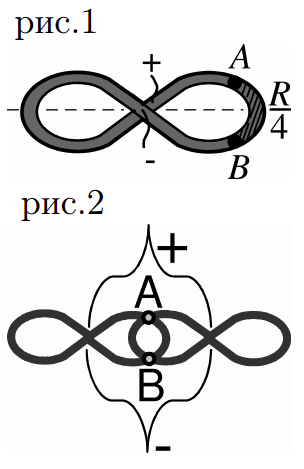
\includegraphics[width=4cm]{42}}

\end{document}
